\documentclass[11pt]{scrartcl}
\usepackage[utf8]{inputenc}
\usepackage{mathtools}
\usepackage{amssymb}

\usepackage{caption}
\usepackage{color}
\usepackage{xcolor}
\usepackage{listings}
\DeclareCaptionFont{white}{\color{white}}
\DeclareCaptionFormat{listing}{\colorbox{gray}{\parbox{\textwidth}{#1#2#3}}}
\captionsetup[lstlisting]{format=listing,labelfont=white,textfont=white}

\usepackage{tikz}
\usetikzlibrary{automata,positioning}

\usepackage{makecell}

\usepackage{changepage}

\usepackage{mwe}

\title{\textbf{1810 Einsendeaufgabe KE 03}}
\author{Gustavo Nunes Martins}

\begin{document}
	\maketitle
	\section*{Aufgabe 1}
	\subsection*{a}
	\begin{tabular}{c|c|c|c|c|c|c}
		  &+&f(&)&1/&x&\$ \\ \hline
		+ & $>$ & $<$ & $>$ & $<$ & $<$ & $>$ \\ \hline
		f(& $<$ & $<$ & $<$ & $<$ & $<$ & $>$  \\ \hline
		) & $>$ & error & $>$ & error & error & $>$  \\ \hline
		1/& $>$ & $<$ & $>$ & $<$ & $<$ & $>$  \\ \hline
		x & $>$ & error & $>$ & error & error & $>$  \\ \hline
		\$& $<$ & $<$ & $<$ & $<$ & $<$ & accept 
	\end{tabular}

Reduktionen sind in grüne Farbe repräsentiert:
\begin{center}
	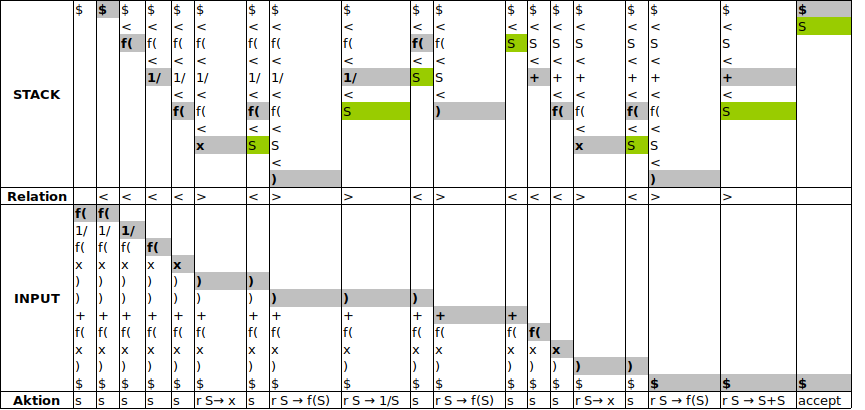
\includegraphics[width=\linewidth]{table.png}
\end{center}
	
	\subsection*{b}
	\section*{Aufgabe 2}
	\subsection*{a}
	17 Zustände sind erforderlich, nämlich:
	\begin{table}[!htbp]
	\begin{tabular}{l|l|l}
		\multicolumn{3}{c}{Zustand 0} \\ \hline
		S' & .S & \$ \\ \hline
		S & .Xa & \$ \\ \hline
		X & .Xb & a,b \\
		& .bYa & a,b \\
	\end{tabular}
	\end{table}

	\begin{table}[!htbp]
		\begin{tabular}[t]{l|l|l}
			\multicolumn{3}{c}{$1: 0 \xrightarrow{S} 1$} \\ \hline
			S' & S. & \$ \\ 
		\end{tabular}
		\begin{tabular}[t]{l|l|l}
			\multicolumn{3}{c}{$2: 0 \xrightarrow{X} 2$} \\ \hline
			S & X.a & \$ \\ \hline
			X & X.b & a,b 
		\end{tabular}
		\begin{tabular}[t]{l|l|l}
			\multicolumn{3}{c}{$3: 0 \xrightarrow{b} 3$} \\ \hline
			X & b.Ya & a,b \\ \hline
			Y & .aXc & a \\ 
			& .a & a \\
			& .aXZ & a 
		\end{tabular}
	\end{table}
	
	\begin{table}[!htbp]
		\begin{tabular}[t]{l|l|l}
			\multicolumn{3}{c}{$4: 2 \xrightarrow{a} 4$} \\ \hline
			S & Xa. & \$ \\ 
		\end{tabular}
		\begin{tabular}[t]{l|l|l}
			\multicolumn{3}{c}{$5: 2 \xrightarrow{b} 5$} \\ \hline
			X & Xb. & a,b \\ 
		\end{tabular}
		\begin{tabular}[t]{l|l|l}
			\multicolumn{3}{c}{$6: 3 \xrightarrow{Y} 6$} \\ \hline
			X & bY.a & a,b \\ 
		\end{tabular}
		\begin{tabular}[t]{l|l|l}
			\multicolumn{3}{c}{$7: 3 \xrightarrow{a} 7$} \\ \hline
			X & .Xb & a,c \\
			& .bYa &a.c \\ \hline
			Y & a.Xc & a \\
			& a. & a \\
			& a.XZ & a 
		\end{tabular}
	\end{table}
		
	\begin{table}[!htbp]
			\begin{tabular}[t]{l|l|l}
				\multicolumn{3}{c}{$8: 6 \xrightarrow{a} 8$} \\ \hline
				X & bYa. & a,b \\ 
			\end{tabular}
			\begin{tabular}[t]{l|l|l}
				\multicolumn{3}{c}{$9: 7 \xrightarrow{X} 9$} \\ \hline
				X & X.b & a,c \\ \hline
				Y & aX.c & a \\ 
				 & aX.Z & a \\ \hline
				Z & .cc & a \\
				& $\varepsilon$ & a 
			\end{tabular}
			\begin{tabular}[t]{l|l|l}
				\multicolumn{3}{c}{$10: 7 \xrightarrow{b} 10$} \\ \hline
				X & b.Ya & a,c \\ \hline
				Y & .aXc & a \\ 
				& .a & a \\ 
				 & .aXZ & a \\
			\end{tabular}
		\end{table}

	\begin{table}[!htbp]
		\begin{tabular}[t]{l|l|l}
				\multicolumn{3}{c}{$11: 9 \xrightarrow{c} 11$} \\ \hline
				Y & aXc. & a \\ \hline
				Z & c.c & a
		\end{tabular}
		\begin{tabular}[t]{l|l|l}
			\multicolumn{3}{c}{$12: 9 \xrightarrow{Z} 12$} \\ \hline
			Y & aXZ. & a \\
		\end{tabular}
		\begin{tabular}[t]{l|l|l}
			\multicolumn{3}{c}{$13: 9 \xrightarrow{b} 13$} \\ \hline
			X & Xb. & a,c \\
		\end{tabular}
		\begin{tabular}[t]{l|l|l}
				\multicolumn{3}{c}{$14: 10 \xrightarrow{Y} 14$} \\ \hline
			X & bY.a & a,c \\
		\end{tabular}
		\begin{tabular}[t]{l}
				$10 \xrightarrow{a} 7$ \\ \hline
		\end{tabular}
	\end{table}
		
		\begin{table}[!htbp]
			\begin{tabular}[t]{l|l|l}
				\multicolumn{3}{c}{$15: 11 \xrightarrow{c} 15$} \\ \hline
				Z & cc. & a \\ 
			\end{tabular}
			\begin{tabular}[t]{l|l|l}
				\multicolumn{3}{c}{$16: 14 \xrightarrow{a} 16$} \\ \hline
				X & bYa. & a,c \\
			\end{tabular}
		\end{table}
	
	\subsection*{b}
	\begin{tabular}{|c|c|c|c|c|c|c|c|c}
 		Zustand& \multicolumn{3}{c}{ACTION} && \multicolumn{4}{c}{GO TO}\\ \hline
 		& a & b & c & \$ & S & X & Y & Z\\ \hline
 		0 & & s3 & & & goto 1 & goto 2 &  & \\ \hline
 		1 & & & & accept &  &  &  & \\ \hline
 		2 & s4 & s5 & & &  &  &  & \\ \hline
 		3 & s7 & & &  &  &  & goto 6 & \\ \hline
 		4 & & & & r $S\rightarrow Xa$ &  &  &  & \\ \hline
 		5 & r $X\rightarrow Xb$ & r $X\rightarrow Xb$& & &  &  &  & \\ \hline
 		6 & s8 & & & &  &  &  & \\ \hline
 		7 & r $ Y \rightarrow  a $ & s10 & & &  & goto 9 &  & \\ \hline
 		8 & r $X \rightarrow bYa$ & r $X \rightarrow bYa$& & &  &  &  & \\ \hline
 		9 & r $Z \rightarrow  \varepsilon $& s13 & s11 & &  &  &  & goto 12\\ \hline
 		10 & s7 & & & &  &  & goto 14 & \\ \hline
 		11 & r $ Y \rightarrow  aXc $& & s15 & &  &  &  & \\ \hline
 		12 & r $ Y \rightarrow  aXZ $& & & &  &  &  & \\ \hline
 		13 & r $ X \rightarrow  Xb $& & r $ X \rightarrow  Xb $ & &  &  &  & \\ \hline
 		14 & s16 & & & &  &  &  & \\ \hline
 		15 & r $ Z \rightarrow  cc $& & & &  &  &  & \\ \hline
 		16 & r $ X \rightarrow  bYa $& & r $ X \rightarrow  bYa $& &  &  &  & \\ \hline
	\end{tabular}
	\subsection*{c}
	(0,babaaaba\$) $\xmapsto{s3}$ (0 b3,abaaaba\$) $\xmapsto{s7}$ (0 b3 a7,baaaba\$) $\xmapsto{s10}$ (0 b3 a7 b10,aaaba\$) $\xmapsto{s7}$ (0 b3 a7 b10 a7,aaba\$) $\xmapsto{r\ Y\rightarrow a}$ (0 b3 a7 b10 Y,aaba\$) $\xmapsto{goto 14}$ (0 b3 a7 b10 Y14,aaba\$) $\xmapsto{s16}$ (0 b3 a7 b10 Y14 a16,aba\$) $\xmapsto{r\ X\rightarrow bYa}$ (0 b3 a7 X,aba\$) $\xmapsto{goto 9}$ (0 b3 a7 X9,aba\$) $\xmapsto{r\ Z\rightarrow \varepsilon}$ (0 b3 a7 X9 Z,aba\$) $\xmapsto{goto 12}$ (0 b3 a7 X9 Z12,aba\$) $\xmapsto{r\ Y\rightarrow aXZ}$ (0 b3 Y,aba\$) $\xmapsto{goto 6}$ (0 b3 Y6,aba\$) $\xmapsto{s8}$ (0 b3 Y6 a8,ba\$) $\xmapsto{r\ X\rightarrow bYa}$ (0 X,ba\$) $\xmapsto{goto 2}$ (0 X2,ba\$) $\xmapsto{s5}$ (0 X2 b5,a\$) $\xmapsto{r\ X\rightarrow Xb}$ (0 X,a\$) $\xmapsto{goto 2}$ (0 X2,a\$) $\xmapsto{s4}$ (0 X2 a4,\$) $\xmapsto{r\ S\rightarrow xa}$ (0 S,\$) $\xmapsto{goto 1}$ (0 S1,\$) $\xmapsto{accept}$ accept

\end{document}